\chapter{关联序列型数据属性隐私推断模型}
\label{chap:inference-attack-on-related-sequenced-data}
\textit{ }

\textit{随着不同机构和个人更加容易获取基因组数据,且这些敏感数据被广泛应用于医疗、保险、寻亲及社交等场景,对数据安全和隐私的担忧也在不断加剧。最近一些实际攻击和真实事件更加增强了对基因组隐私的担忧。为了证实并披露在序列型数据属性隐私方面,个人共享基因数据也会大量泄漏他人属性隐私的机理。本章针对家庭成员间基因序列数据共享会造成的隐私泄露问题展开研究,并证实了上述问题会变得更糟。本章中,利用因子图和置信传播算法针对亲属间的基因序列属性隐私建立分析推断敌手模型和分析算法亲属基因组属性隐私推断攻击的准确性。该模型考虑了单核苷酸多态性间高阶相关性,利用公开DNA参照数据集和全基因组关联研究(GWAS)目录数据,提高了推断攻击模型的属性隐私分析强度。该模型的敌手隐私分析强度通过第~\ref{chap:entropy-metric-model}章所提出的隐私度量框架,将隐私损失量作为评价指标进行了量化。实验结果表明,所提出的攻击更适合于高密度基因组数据隐私推断,且具有较少的不正确性、不确定性和更多隐私损失,显著提高了属性隐私的推断能力。}

\section{概述}
得益于生物技术的快速发展,人们可以廉价地对DNA进行测序,并很容易地将自己的基因组数据分享给他人。越来越多的人为了不同的目的(如精准基因组医学、全球基因组研究、了解个人遗传疾病情况、寻找祖先和亲属或者仅仅为了娱乐),将其基因组数据共享。政府、研究机构、医疗组织、健康相关网站和在线社交网络已收集了成千上万个人基因组数据,其中大部分数据都可以下载或在网上公开共享。

尽管网上的大部分基因组数据都是匿名化的,但是这些数据都可以被去匿名化重新识别~\cite{greenbaum2008genomic,humbert2015de}。甚至即使一个个体在共享其基因组数据之前隐藏了部分数据,也能重构隐藏部分的基因序列数据,并了解私人疾病和特征信息。因此,共享基因组数据的所有者可能面临来自雇主或保险公司的歧视风险。此外,超过99.9\%的基因组数据对人类来说相同的,在亲属中具有相同基因组数据的占比更高。因此,若一个人暴露了其基因组数据,就会导致其基因组隐私和其亲属的基因组隐私受到威胁,如亲属关系隐私和家族身份隐私~\cite{rohlfs2012familial}。


实际情况会更糟,最近的新闻报道称,警方通过开源遗传数据库中的家族成员基因组数据,发现并逮捕了金州杀手,该罪犯在1974年至1986年期间在加州造成12人死亡和至少50起强奸案。这一消息引起了人们对基因隐私的极大关注。若有亲属参与了基因研究或在网上分享了他们自己基因,你应该担心自己的隐私吗?是否有可能从某人的亲属基因数据中重构该人的基因组数据?通过这种方式可以重构多少基因信息?通过亲属的基因数据可以泄露该人的多少基因隐私量?

基于最近的研究和真实的新闻报道,本文针对相互关联序列型数据的属性隐私提出了一种敌手模型和概率推断方法。该模型是针对亲属基因组隐私的高精度推断攻击,并利用前文提出的度量方法对隐私和隐私分析推断攻击强度进行了量化。该攻击模型旨在从公开的基因组数据和网站上的亲属基因组信息中推断出个人的基因组属性隐私信息。提出了一个统一的敌手模型和一个基于离散隐Markov模型、高密度参考数据集和GWAS目录的推断攻击框架,并利用因子图和置信传播算法实现了基因属性隐私推断攻击。与Humbert和Deznabi等~\cite{deznabi2018inference}的工作相比,我们的贡献是:

\begin{enumerate}
	\item 提出了一种利用9种公开的和观测到的家庭成员基因组数据进行推断攻击的敌手模型,攻击者的目标是推断被攻击者的基因组属性值、遗传疾病信息和遗传特征信息。
	\item 提出了利用高密度参照数据集IMPUTE2~\cite{howie2014impute2}中SNP序列的相关性进行推断攻击,并设计了一个扩展因子图和基于置信传播的基因属性隐私推断攻击算法。
	\item 利用互信息度量所提出的推断攻击强度,量化基因组隐私,刻画攻击者对属性隐私不确定性的降低和被攻击者基因属性隐私损失的增加。
	\item 针对被攻击者的基因属性隐私推断,得到了非常高的准确性和更低的不确定,比以前的工作更加适用于高密度基因组数据隐私分析。
\end{enumerate}

\section{相关背景知识}
\label{sec:backgrounds}
在本节中,我们简要介绍遗传学的背景和基于因子图的置信传播。

\subsection{基因组信息}

人类基因组被编码为23个染色体对中的DNA,并包含约30亿个核苷酸对。 每个染色体都是双螺旋结构,由两个互补的核苷酸核苷酸(A,T,G,C)聚合链组成。人类 99\% 的DNA信息是一样的, 仅有基因组的0.5\% 是显着的差异。当基因组序列中的单个核苷酸 (A, T, C, 或 G) 在遗传过程中发生变化时,DNA序列产生变异。

单核苷酸多态性 (Single-Nucleotide Polymorphism, SNP)是在基因组中特定位置出现的单个核苷酸变体,其中每个变体在种群中都以一定程度的概率存在。 对于每个SNP,存在三种可能的基因型:(i) 普通等位基因是纯合子, (ii) 对于较不常见的等位基因是杂合的,(iii) 稀有等位基因纯合子; 通常分别编码为0、1和2。 SNP经常与疾病和个人特征有关, SNPedia和GWAS Central是支持全基因组关联研究 (GWAS) 中的个人基因组注释,解释和分析的数据库。

孟德尔遗传定律表明一个人的SNP都是是独立于其父母继承的。 对于一个SNP位点,一个等位基因来自父亲,一个等位基因来自母亲,概率为0.5。 本章工作依照文献~\cite{humbert2013addressing}和~\cite{deznabi2018inference}中的模型使用该定律,参见图~\ref{fig:Mendelian-law}中的概率模型。

\begin{figure}[htbp]
	\centering
	\includegraphics[width=0.6\linewidth]{./figures/Mendelian-law.jpg}
	\centering
	\caption{SNP孟德尔遗传定律概率模型}\label{fig:Mendelian-law}
\end{figure}

连锁不平衡(Linkage Disequilibrium,LD)由两个或多个基因座上等位基因的对应关系或非随机关系定义。 研究人员提出了各种方法来描述SNP之间的相关性, 这些方法中的三种是最新的选择,它们分别使用公开的等位基因频率和连锁不平衡,基因型数据集和遗传重组率~\cite{samani2015quantifying} 。通过使用高密度单倍型参照数据集、遗传重组率、离散隐Markov链模型和Markov链蒙特卡洛采样策略,提出了IMPUTE2~\cite{howie2014impute2},一种缺失基因型的概率估算方法。 与在文献~\cite{humbert2013addressing,humbert2017quantifying}中使用的成对连锁不平衡和在文献~\cite{deznabi2018inference} 中使用的简单(隐藏) Markov链不同,在本章工作中使用IMPUTE2中的方法作为基因属性隐私分析推测的相关性和采样算法。

\subsection{置信传播}

置信传播~\cite{kschischang2001factor} 是一种用于在图形模型上进行推断的消息传递算法,且在贝叶斯网络和Markov随机域上运行良好。 它在观测到的节点上有条件地评估未观测到的节点的边缘概率。 它在具有近似结果的循环因子图和具有精确结果的无循环因子图上均具有良好的性能。 置信传播在人工智能和信息论中被广泛使用。 在本章中,使用 SumProductLab作为基本开放工具来实现针对所提出的推断攻击的置信传播算法。

\section{关联基因序列数据隐私分析敌手模型}
\subsection{数据模型}
对于特定的家庭,有~$~n~$~个家庭成员 ~$~S=\{s_1,s_2,...,s_n\}$~,以及该家庭的亲属结构图 ~$~T=\{S,R\}$~ ,其中 ~$~S~$~ (是家庭成员的集合) 赋予为 ~$~T~$~ 的顶点, 而 ~$~R~$~ (是家庭成员关系的集合,若 ~$~s_i~$~ 是 ~$~s_j~$~ 的父母,则 ~$~r_{i,j}=1~$~) 赋予为 ~$~T~$~ 的边。 假设一个人的SNP集为 ~$\mathbf{x}=(x_1,x_2,...,x_m)~$~ 并具有 ~$~m~$~ 个SNP, 其中 ~$~x_i \in \{0,1,2\}$~ (特定的SNP ~$~x_i~$~ 具有 ~$~"BB"~$~,~$~"Bb"~$~ 和 ~$~"bb"~$~ 的基因型, 可以分别用0、1和2来赋值), 因此 ~$~s_i~$~ 的SNP集可以赋予为 ~$\mathbf{x}_i=(x_{i,1},x_{i,2},...,x_{i,m})~$~。令矩阵 ~$\mathbf{X}$~ 代表整个家族的所有SNP,则

\begin{equation}
\mathbf{X}=
\left[
\begin{matrix}
x_{1,1} & x_{1,2} & ...    & x_{1,m} \\
x_{2,1} & x_{2,2} & ...    & x_{2,m} \\
\vdots  & \ldots  & \ldots & \vdots  \\
x_{n,1} & x_{n,2} & ...    & x_{n,m}
\end{matrix}
\right]
\end{equation}

对于某个族群的某个人,例 CEU~\cite{auton2015a}, 一个SNP的概率分布由等位基因频率决定。  因此,某个族群中任意人的SNP ~$~x_i \in \mathbf{x}$~ 服从该等位基因座的等位基因分布 ~$\mathbf{p}_i~$~ ,其中 ~$\mathbf{p}_i=\{p_{i,0},p_{i,1}, p_{i,2}\}$~, ~$~p_{i,0}+p_{i,1}+p_{i,2}=1~$~。然后设任意个体的SNP序列为 ~$\mathbf{x}$~, 有

\begin{equation}
\left(
\begin{matrix}
x_1          & x_2 & ... & x_m \\
\mathbf{p}_1 & \mathbf{p}_2 & ... & \mathbf{p}_m
\end{matrix}
\right)
\end{equation}

由于减数有丝分裂和DNA重组,一个人的SNP之间存在某些关联关系,其中成对的连锁不平衡是SNP最常见和最基本的关系, 若 ~$~x_i~$~ 和 ~$~x_j~$~ 相互关联,则存在系数 ~$~f_{i,j}$~ 。基于成对连锁不平衡,可以通过总体SNP集合来训练一些其他高阶关系。

此外,一个人的SNP决定了其自己的外在特征和疾病。 设 ~$\mathbf{t}$~ 为可观测到的性状, ~$\mathbf{d}$~ 为与基因组有关的疾病。  性状 ~$~t_i \in \mathbf{t}$~ 的表型与子集 ~$\mathbf{x}t_i \subseteq \mathbf{x}$~ 有关, 疾病 ~$~d_i \in \mathbf{d}$~ 与子集 ~$\mathbf{x}d_i \subseteq \mathbf{x}$~ 有关。 人类表型本体论项目(Human Phenotype Ontology project)~\cite{koehler2014human}和GWAS目录( GWAS Catalog)~\cite{macarthur2017the}中发布了唯一的SNP特征和SNP疾病关联关系数据。


在实际中,往往部分数据已知而部分数据未知。SNP序列数据是敏感的隐私数据,人们总是在共享或发布基因组数据之前隐藏一些SNP或在SNP中添加噪音。 加噪的方式会使基因组数据杂乱而导致医学研究和精准医疗获得意想不到的结果,因此人们通常只是隐藏了不想共享的部分SNP序列取值。 因此,家族成员的已知SNP赋为 ~$\mathbf{X}_K~$~, 未知SNP赋为 ~$\mathbf{X}_U~$~,其中 ~$\mathbf{X}_K \perp\mathbf{X}_U~$~ 和 ~$\mathbf{X}_K \cup \mathbf{X}_U = \mathbf{X}$~; 家庭成员的已知特征是 ~$\mathbf{T}_K~$~, 未知特征是 ~$\mathbf{T}_U~$~; 家庭成员的已知基因组疾病是 ~$\mathbf{D}_K~$~, 未知基因组疾病是 ~$\mathbf{D}_U~$~。同样, ~$\mathbf{T}_K \perp \mathbf{T}_U~$~, ~$\mathbf{D}_K \perp \mathbf{D}_U~$~, ~$\mathbf{T}_K \cup \mathbf{T}_U = \mathbf{T}$~, 以及 ~$\mathbf{D}_K \cup \mathbf{D}_U = \mathbf{D}$~, 其中 ~$\mathbf{T}$~ 表示家庭成员的可观测基因组特征, ~$\mathbf{D}$~ 表示家庭成员的遗传疾病。 ~$\mathcal{F}_T(x_i^F,x_i^M,x_i^C)~$~ 是孟德尔遗传概率函数,其中 ~$~(F,M,C)~$~ 分别代表父亲,母亲和孩子。~$\mathbf{P}=\{p_i: i \in \mathbf{x}\}$~ 表示 ~$\mathbf{x}$~ 中SNP的次要等位基因概率(或 MAF) 的集合。 ~$\mathbb{T}=\{(t_i,rt_{SNP序列}(t_i): t_i \in \mathbf{t}\}$~ 表示遗传性状与SNP之间的关系,其中 ~$~rt_{SNP序列}(t_i)~$~ 是由该集合的元素确定的 ~$~t_i~$~ 的SNP集,而 ~$~rt_{SNP序列}(t_i) \subseteq \mathbf{x}$~。 ~$\mathbb{D}=\{(d_i,rd_{SNP序列}(d_i): d_i \in \mathbf{d}\}$~ 代表遗传疾病与SNP之间的关系,其中 ~$~rd_{SNP序列}(d_i)~$~ 是由该集合的元素决定的 ~$~d_i~$~ 的SNP集,而 ~$~rd_{SNP序列}(d_i) \subseteq \mathbf{x}$~。 ~$\mathbb{P}=\{p_{d_i}: d_i \in \mathbf{d}\}$~ 代表遗传疾病的患病率。

\subsection{敌手模型}

本节构建类似于Humbert等工作~\cite{humbert2013addressing}(第3.1节)中的敌手模型。 敌手是由其目标(s), 攻击方法(s) 和背景知识来定义的。本章中,敌手的目的是通过使用 (i) 观测到的一个或多个家庭成员的基因组数据 (即 SNP序列),  (ii) 观测到的一个或多个家庭成员的基因组相关特征和疾病, (iii) 家庭的血统结构, (iv) 繁殖规则,特别是孟德尔遗传定律, (v) 核苷酸的次要等位基因频率 (MAFs) 或等位基因频率, (vi) SNP之间的族群LD值, (vii) 族群的SNP, (viii) GWAS目录,以及 (ix) 遗传疾病的发病率等信息,推断被攻击者的SNP,身体特征和疾病。值得注意的是,(i)-(iii) 可以从基因组共享网站 (如openSNP.org)和开放社交网络(如facebook.com 和 PatientsLikeMe.com) 收集; (iv) 是遗传学的公共信息; (v)-(vii) 是可以从基因组研究网站 (即 internationalgenome.org) 收集的基因组公共信息; (viii) 和 (ix) 可以从GWAS目录项目和政府统计局 (如 CDC)收集。

敌手意图通过观测有关家庭的各类基因组信息和公开基因信息来推断多个家庭成员的多个SNP,多个特征和多种疾病。 尽管文献~\cite{humbert2013addressing} 中提到了其他类型的攻击方法,也可以通过这种攻击来进行攻击。 这种攻击可以表述为类似于文献~\cite{humbert2013addressing,humbert2017quantifying,deznabi2018inference}的统计推断问题。

\subsection{推断模型}

为了使本章的攻击者模型有效并提高基因序列属性隐私分析推断攻击的强度,本节分析以前的工作方法和本章工作的研究动机,并阐明本章进行亲属基因组隐私分析的推断攻击改进途径。

Humbert等~\cite{humbert2013addressing}在CCS'13中提出了亲属基因组隐私推断攻击的原始工作。 文献~\cite{humbert2013addressing}的工作证实了基因组和疾病隐私受到亲属基因组隐私泄露的威胁, 作者采用了5种观测和公开信息 (即家庭成员的SNP,所观测家庭的血统结构,繁殖规则,MAF和成对LD值)。 在文献~\cite{humbert2017quantifying}中, Humbert等用亲属的表型扩展了~\cite{humbert2013addressing} 的工作,并获得了一些新的结果。
在文献~\cite{deznabi2018inference} 中, Deznabi等改进了~\cite{humbert2013addressing} 的工作,借助SNP之间的高阶相关性,采用了具有重组模型的高阶Markov链和隐Markov链~\cite{marchini2007newa,samani2015quantifying},获得了良好的隐私分析结果。
由此可知,使用的可观测性和公共基因组信息越多,使用的SNP越接近现实相关性,从亲属的基因组数据中可以推断出的被攻击者基因隐私信息就越多。

如所提出的敌手模型所述,我们将采用9种可观测和公开的基因组信息,可观测亲属的可观测疾病和特征信息,族群的SNP(如来自1000基因组计划(1000 Genomes Project)的单倍体参照数据集) 和遗传疾病的流行率(如CDC.gov和snpedia.com的GWAS目录) 。 另一方面,我们将在SNP之间使用一些新的相关模型,即IMPUTE2中提出的带有Markov链蒙特卡洛斯采样的离散隐Markov模型~\cite{howie2014impute2}。IMPUTE2的最初目的是提高1000基因组计划的质量,它比朴素的隐式Markov模型~\cite{marchini2007newa,samani2015quantifying}更具优势。在这里,我们将采用这些方法来进行基因序列属性隐私分析,并改进亲属基因组隐私分析推断攻击效果 。

此外, 文献~\cite{humbert2013addressing,humbert2017quantifying,deznabi2018inference}直接从观测到的基因组数据推断出被攻击者的基因组隐私。 本章我们将基因数据属性隐私推断攻击分为两个阶段。在第一阶段,利用IMPUTE2从观测到的亲属SNP,单倍体参照数据集,LD值和MAF值等推断出亲属未观测到的SNP序列值。 有关IMPUTE2的更多详细信息,请参见文献~\cite{howie2014impute2}。
在此阶段,我们还将考虑每个父母与孩子之间的关系。在第二阶段,使用推断的亲属基因组数据和敌手模型中确定的信息来推断被攻击者的SNP值并量化基因组隐私。 在此阶段将使用置信传播算法来计算被攻击者SNP值的近似概率分布。

\section{基因属性隐私分析框架及方法}
\label{sec:inference-attack}

\subsection{属性隐私分析概述}

\begin{figure}[htbp]
	\centering
	\includegraphics[width=0.95\linewidth]{./figures/attack-framework.png}
	\centering
	\caption{亲属基因组属性隐私分析推断框架}\label{fig:attack-framework}
\end{figure}

如图~\ref{fig:attack-framework}所示,敌手拥有一些背景知识信息,且观测到有关该家庭的一些基因组信息,然后他意图推断被攻击者的基因组相关属性隐私。 我们将攻击分为三个阶段:a)建立可以通过背景知识增强攻击的高阶相关模型; b)推断有关被攻击者的私人信息,包括敌手尚未收集到的隐私SNP,私人特征和疾病; c)量化推断获取的隐私信息量。

\subsection{基因属性隐私分析模型}
旨在推断目标SNP值,特征和疾病的存在的攻击可以公式化为计算未知变量~$\mathbf{X}_U~$~,~$\mathbf{T}_U~$~和~$\mathbf{D}_U~$~的边缘概率分布,
给定观测值(~$\mathbf{X}_K~$~,~$\mathbf{T}_K~$~和~$\mathbf{D}_K~$~和家族结构)和背景知识(孟德尔遗传定律函数~$\mathcal{F}_T(x_i^F,x_i^M,x_i^C)~$~),次要等位基因概率~$\mathbf{P}$~,性状与SNP之间的关系~$\mathbb{T}$~,疾病与SNP之间的关系~$\mathbb{D}$~,遗传疾病的患病率~$\mathbb{P}$~,重组模型~$\mathbf{F}$~的公式以及种群的SNP)。 因此,利用联合概率分布函数可以获得未知变量的边缘概率分布。

\begin{equation}\label{eq:joint-pro}
\begin{aligned}
p(\mathbf{X}_U, \mathbf{T}_U, \mathbf{D}_U | \mathbf{X}_K, \mathbf{T}_K, \mathbf{D}_K, T, \mathcal{F}_T(x_i^F,x_i^M,x_i^C), \mathbf{P}, \mathbb{T}, \mathbb{D}, \mathbb{P}, \mathbf{F})
\end{aligned}
\end{equation}

假设~$\hat{\mathbf{X}_U}$~是~$\mathbf{X}_U~$~的推断值,则可以将公式~\ref{eq:joint-pro}解析为两步:1)公式~\ref{eq:joint-pro}和2)公式~\ref{eq:joint-pro-Tu}和公式~\ref{eq:joint-pro-Du}

\begin{equation}\label{eq:joint-pro-Xu}
p(\mathbf{X}_U | \mathbf{X}_K, \mathbf{T}_K, \mathbf{D}_K, T, \mathcal{F}_T(x_i^F,x_i^M,x_i^C), \mathbf{P}, \mathbb{T}, \mathbb{D}, \mathbb{P}, \mathbf{F})
\end{equation}

\begin{equation}\label{eq:joint-pro-Tu}
p(\mathbf{T}_U |\hat{\mathbf{X}_U}, \mathbf{X}_K, \mathbf{T}_K, \mathbf{D}_K, T, \mathcal{F}_T(x_i^F,x_i^M,x_i^C), \mathbf{P}, \mathbb{T}, \mathbb{D}, \mathbb{P}, \mathbf{F})
\end{equation}

\begin{equation}\label{eq:joint-pro-Du}
p(\mathbf{D}_U |\hat{\mathbf{X}_U}, \mathbf{X}_K, \mathbf{T}_K, \mathbf{D}_K, T, \mathcal{F}_T(x_i^F,x_i^M,x_i^C), \mathbf{P}, \mathbb{T}, \mathbb{D}, \mathbb{P}, \mathbf{F})
\end{equation}


然后,若将家庭成员~$~i~$~的SNP ~$~j~$~的边缘分布表示为~$~p(x_{ij})~$~,则~$\mathbf{X}_U~$~的每个变量的边缘概率分布可以得到为

\begin{equation}\label{eq:joint-pro-Xu2}
\begin{aligned}
p(x_{ij})= \sum_{\mathbf{X}_U/\{x_{ij}\}} p(\mathbf{X}_U | \mathbf{X}_K, \mathbf{T}_K, \mathbf{D}_K, T,  \mathcal{F}_T(x_i^F,x_i^M,x_i^C), \mathbf{P}, \mathbb{T}, \mathbb{D}, \mathbb{P}, \mathbf{F})
\end{aligned}
\end{equation}


传统上,由于复杂度随项数的增加而呈指数增长,因此无法计算公式~\ref{eq:joint-pro-Xu2}。实际上,一个人拥有数百万个SNP,并具有许多性状和基因组疾病,从而使计算不可行。


基于因子图的方法是一种评估概率~\cite{kschischang2001factor}的有效方法。此外,由于SNP之间的重组和相关在染色体中是部分的,因此有可能将SNP,性状和疾病分为不同的分区。 因此,我们将联合概率分布分解为一组局部函数,每个函数通过将其作为变量来表示SNP序列,家庭成员,性状和疾病之间的依赖关系。 然后,通过在因子图上启动置信度传播,可以线性复杂度获得边缘概率分布。


在这里,我们为计算建立一个因子图。该图具有两种类型的节点(变量节点和因子节点)和连接节点的边。与~\cite{humbert2013addressing,humbert2017quantifying,deznabi2018inference}相似,在此因子图中设置了每个SNP ~$~x_{i,j}$~的变量节点~$~(\in \mathbf{X}$~,~$~i~$~表示家庭成员ID,~$~j~$~表示家庭成员~$~i~$~的SNP ID)。但是本章模型使用四种类型的因子节点和~\cite{deznabi2018inference}:(i)\emph{家族因子节点},代表家族关系(关于孩子和父母)和繁殖,(ii)\emph{重组模型相关因子节点},代表之间的重组模型相关性SNP,正如我们在第二节中所述II,它包含比其他类型的高阶相关性更多的信息,(iii)\emph{特征因子节点}代表SNP与个体特征之间的关系,以及(iv)\emph{疾病因素节点},代表SNP与个体基因组疾病之间的关系。在这里,对于\emph{相关节点},与~\cite{humbert2013addressing}和~\cite{deznabi2018inference}的工作不同,我们利用重组模型来表示SNP的相关性。如Marchini等~\cite{marchini2007newa}和Samani等~\cite{samani2015quantifying}所示,重组模型在验证和校正基因型标记~\cite{marchini2007newa}处的数据方面具有良好的性能,且在预测隐藏的SNV方面具有更好的性能,因为它包含重组和突变因子~\cite{samani2015quantifying}。这项工作,我们将其直接用于构建因子图,并推断出与亲属关系相关的基因组隐私。此外,由于在工作中采用了GWAS目录和遗传疾病的患病率,因此我们用\emph{特征因子节点}和\emph{疾病因素节点}代替了~\cite{deznabi2018inference}中的\emph{表型因子节点} 来形成因子图。除了观测家族成员的特征和疾病,GWAS目录还可以分别提供SNP与特征和疾病之间的更多相关性。而且遗传疾病的患病率可以提供一些其他信息来推断SNP的价值。 GWAS中的常识是,疾病和性状与SNP序列~\cite{manolio2008a}有关,某些复杂的疾病由多个SNP序列和其他因素~\cite{climer2014a}决定。我们提出的因素图如图~\ref{fig:factor-graph}所示,变量之间的联系和因子节点描述如下。

\begin{itemize}
	\item 每个变量节点~$~x_{i,j}$~具有其家族因子节点~$~f_{i,j}$~并已连接。 且,若~$~k~$~是家庭中~$~i~$~的父母,则~$~x_{k,j}$~(~$~ k \neq i~$~)也连接到~$~x_{i,j}$~。 若所观测到的家庭中父亲或母亲都没有~$~i~$~,则因子节点~$~f_{i,j}$~的程度为1; 若只有~$~i~$~现在的父亲或母亲,则因子节点~$~f_{i,j}$~的度数为2; 若被观测家庭中有双亲~$~i~$~,则该度数为3。 如图3中的示例所示,孩子的家庭因子节点的度数为3,因为他的父母都在这里,而父母的家庭因子节点的度数均为1,因为父亲或母亲的父母都不是 出现在被观测家庭中。
	\item 集合~$\mathbf{C}$~中的变量节点连接到重组模型相关因子节点~$~rf_{i,\mathbf{C}}$~。 由于我们使用重组模型来训练SNP之间的相关性,因此所有SNP都可以视为与重组能力相关。 在这里,设置~$\mathbf{C}$~等于~$\mathbf{x}$~,其中包括一个人的所有SNP。 另一方面,Markov假设可以提高效率。 我们在评估步骤中使用基于Markov的计算。
	\item 若~$\mathbf{T}_{i,\alpha}$~中的SNP与特征~$~t_{\alpha}$~( ~$~t_{\alpha} \in \mathbf{t}$~)相关联,则集合~$\mathbf{T}_{i,\alpha}$~中的家族成员~$~i~$~的可变节点连接到特征因子节点~$~tf_{i,\alpha}$~。 ~$\mathbf{T}_{i,\alpha}$~和 ~$\mathbf{T}_{j,\alpha}$~ (~$~i \neq j~$~)的SNP具有相同的基因座集合。 这意味着对于不同个体的特定特征,相关SNP的位点是相同的。 ~$\mathbf{T}_{i,\alpha}$~中的SNP数量可能大于1。换句话说,一个给定的性状与一个以上的SNP相关。 另外,一个SNP也可能与一个以上的性状相关。 有时,家族成员已经观测到某些特征,有时没有。
	\item 若~$\mathbf{D}_{i,\beta}$~中的SNP与遗传疾病~$~d_{\beta}$~(~$~d_{\beta} \in \mathbf{d}$~)相关,则~$\mathbf{D}_{i,\beta}$~组中家族成员~$~i~$~的可变节点连接到性状因子节点~$~df_{i,\beta}$~。 类似地,可能有不止一种SNP与给定的遗传疾病相关。 一种SNP也可能与一种以上疾病有关。有时,已经从家族成员身上观测到了某些疾病,而有时则没有。值得注意的是,对于特定疾病,即使相关SNP的位点对于不同的个体而言都是相同的,该疾病的当前结果也有所不同,因为该疾病也可能受到其他因素的影响。
	
\end{itemize}


若条件依赖性是通过使用观测到的信息和公共信息给出的,则因子图中变量节点~$~p(\mathbf{X}_U | \mathbf{X}_K, \mathbf{T}_K,\mathbf{D}_K,~$~ ~$~T, \mathcal{F}_T(x_i^F, x_i^M, x_i^C), \mathbf{P}, \mathbb{T}, \mathbb{D}, \mathbb{P}, \mathbf{F})~$~的全局分布可以分解为几个局部函数的产生。 每个局部函数都有一个来自~$\mathbf{X}$~的变量节点子集作为参数。


其中~$~Z~$~是标准化常数,~$\Theta(x_{i,j})~$~是~$\mathbf{T}$~中~$~i~$~的父代的SNP ~$~j~$~值的变量集,~$\Psi(i,\alpha)~$~是个体~$~i~$~与特征~$\alpha~$~相关的SNP值的变量集,~$\Phi(i,\beta)~$~是变量集 ~$~i~$~个体的SNP值与疾病B相关。

公式~\ref{eq:variable-message}的因式分解基于置信传播的规则,变量和因子节点之间传递的信息可用于构造迭代置信传播算法,以计算全局边缘概率分布。 令~$\mathbf{X}^v=\{x_{i,j}^v: i\in \mathbf{S}, j \in \mathbf{SID}\}$~是表示算法在~$~v^{th}$~迭代时变量节点值的变量集合。 我们将消息描述如下。

\begin{itemize}
	\item 消息~$\mu_{i\rightarrow k}^{v}(x_{i,j}^{v})~$~(从变量节点~$~i~$~到因子节点~$~k~$~)表示了 ~$~x_{i,j}^v=l~$~ (~$~l \in {0,1,2}$~),在~$~v^{th}$~迭代中。
	\item 从家族因子节点到变量节点的消息表示为~$\lambda_{k \rightarrow i}^v(x_{i,j}^v)~$~,表示~$~x_{i,j}^v=l~$~ (~$~l \in {0,1,2}$~),在~$~v^{th}$~迭代中,给定~$\mathcal{F}_{R}(x_{M,j},x_{F,j}, x_{C,j})~$~,~$\mathbf{P}$~以及与单个~$~i~$~的相应家庭因子节点关联的家庭成员的SNP的~$~j~$~值。
	\item 从重组模型相关因子节点到变量节点的消息表示为~$\beta_{k \rightarrow i}^v(x_{i,j}^v)~$~,表示~$~x_{i,j}^v=l~$~ (~$~l \in {0,1,2}$~),在~$~v^{th}$~迭代中,基于SNP之间基于建模重组率的相关性。
	\item 从特征因子节点到变量节点的消息表示为~$\varphi_{k \rightarrow i}^v(x_{i,j}^v)~$~,表示在~$~v^{th}$~迭代中 ~$~x_{i,j}^v=l~$~ (~$~l \in {0,1,2}$~)的概率 ,给出单个~$~i~$~的特征~$~t_k~$~以及相应特征与SNP ~$~j~$~的关联~$\mathbb{T}$~。
	\item 从疾病因子节点到变量节点的消息表示为~$\tau_{k \rightarrow i}^v(x_{i,j}^v)~$~,表示在给定疾病~$~d_k~$~的情况下,在~$~v^{th}$~迭代中~$~ x_ {i,j} ~$~(~$~ l ~$~)的概率。 个体~$~i~$~和相应疾病的~$\mathbb{D}$~与SNP ~$~j~$~的关联,以及疾病的患病概率分布~$\mathbb{P}$~。
	
\end{itemize}

\subsection{家族基因属性隐私分析示例}

\begin{figure}[htbp]
	\centering
	\includegraphics[width=0.95\linewidth]{./figures/factor-graph.png}
	\centering
	\caption{三个成员家族3个SNP的因子图示例}\label{fig:factor-graph}
\end{figure}

为了更好地理解该公式,我们仅以母亲,父亲和孩子以及3个SNP为例选择一棵家谱。如图3所示,为三人组构建了一个因子图,且SNP在因子图中表示,其中子图 (a) 是三个成员家族的结构图;(b)是因子图中的符号;(c) 是因子图和节点之间传递的消息。在因子图中,~$~i=1~$~,~$~i=2~$~和~$~i=3~$~分别表示母亲,父亲和孩子,这3个SNP分别表示为~$~j=1~$~,~$~j=2~$~和~$~j=3~$~。在这里,我们描述了表示母亲的第一个SNP的变量节点(~$~x_{1,1}$~),孩子的家庭因素节点(~$~f_{3,1}$~)和重组模型之间的消息交换母亲的相关因子节点(~$~rf_{1,\mathbf{C}}$~),母亲的特征因子节点(~$~tf_{1,\alpha}$~)和母亲的疾病因子节点(~$~df_{1,\beta}$~)。我们假设所有SNP都包含在集合~$\mathbf{C}$~中,特征~$\alpha~$~与SNP 1和2相关,而疾病~$\beta~$~与SNP 2和3相关。在图~\ref{fig:factor-graph}中(c),通过置信传播算法迭代变量节点和因子节点之间的消息,并在每次迭代中更新对~$\mathbf{X}_U~$~中目标SNP值的置信,直到收敛为止。我们分别用~$~i~$~,~$~k~$~,~$~z~$~,~$~s~$~和~$~t~$~表示变量和因子节点~$~x_{1,1}$~,~$~f_{3,1}$~,~$~rf_{1,\mathbf{C}}$~,~$~tf_{1,\alpha}$~和~$~df_{1,\beta}$~。


\emph{来自变量节点的消息。}算法由变量节点启动,生成并发送消息到邻居。变量节点~$~i~$~通过乘以从邻居那里收到的除家族因子节点~$~k~$~之外的所有信息,生成消息~$\mu_{i \rightarrow k}^v(x_{1,1}^v~$~。 可以类似地生成到其他邻居的变量节点~$~i~$~,然后在~$~v^{th}$~迭代中从变量节点~$~i~$~到家庭因子节点~$~k~$~的消息是

\begin{equation}\label{eq:variable-message}
\mu_{i \rightarrow k}^v(x_{1,1}^v)= \frac{1}{Z} \times
%\prod_{w \in \{f_{1,1}\}} \lambda_{w \rightarrow i}^{v-1}(x_{1,1}^{v-1}) \times
\beta_{z \rightarrow i}^{v-1}(x_{1,1}^{v-1}) \times
\varphi_{s \rightarrow i}^{v-1}(x_{1,1}^{v-1})
\end{equation}

其中~$~Z~$~是归一化常数,对每个变量节点的每个邻居重复此计算。若已知~$~x_{1,1}$~的值,则消息~$\mu_{i \rightarrow k}^v(x_{1,1}^v =l)~$~(~$~l\in \{0,1,2\}$~)将为常数1。在这里,我们不使用消息~$\lambda_{k \rightarrow i}^{v-1}(x_{1,1}^{v-1})~$~和\\ ~$\varphi_{t \rightarrow i}^{v-1}(x_{i,j}^{v-1})~$~生成~$\mu_{i \rightarrow k}^v(x_{1,1}^v)~$~,因为在示例中它们没有意义。值得注意的是,若图中包含母亲的父母,则应使用消息~$\lambda~$~生成~$\mu_{i \rightarrow k}^v(x_{1,1}^v)~$~; 若有任何疾病与~$~x_{1,1}$~相关,则还应使用来自那些疾病因子节点的消息~$\varphi~$~。

\emph{来自家庭因素节点的消息。}从家庭因子节点~$~k~$~到~$~v^{th}$~处变量节点~$~i~$~的消息,使用置信传播的原理形成迭代

\begin{equation}
\label{eq:familial-message}
\lambda_{k \rightarrow i}^v(x_{1,1}^v) =  \sum_{\{x_{2,1},x_{3,1}\}}f_{3,1}(x_{1,1},\Theta(x_{1,1}),\mathcal{F}_{R}(x_{M,j},x_{F,j}, x_{C,j},\mathbf{P}) 
\times \prod_{y\in \{x_{2,1},x_{3,1}\}} \mu_{y \rightarrow k}^v(x_{1,1}^v)
\end{equation}

在公式~\ref{eq:familial-message}中,~$~f_{3,1}(x_{1,1},\Theta(x_{1,1}),\mathcal{F}_{R}(x_{M,j},x_{F,j}, x_{C,j},\mathbf{P})~$~与~$~p(x_{1,1}| x_{2,1},x_{3,1},\mathcal{F}_{R}(x_{M,j},x_{F,j}, x_{C,j},\mathbf{P})~$\\成正比,且可以通过图~\ref{fig:Mendelian-law}所示的继承定律进行计算。若特定SNP的程度为1,则家族因子节点仅取决于其次要等位基因频率 相应的SNP。 对每个家庭因素节点的每个邻居重复此计算。


\emph{来自重组模型相关因子节点的消息。} 在~$~v^{th}$~迭代中形成了从重组模型相关因子节点~$~z~$~到变量节点~$~i~$~的消息。

\begin{equation}\label{eq:relavtes-information}
\beta_{k \rightarrow i}^v(x_{1,1}^v) = \sum_{\{x_{1,2},x_{1,3}\}}rf_{1,\mathbf{C}}(x_{1,1},x_{1,2},x_{1,3},\mathbf{F},) \times  \prod_{y \in \{2,3\}} \mu_{x_{1,y} \rightarrow k}^v(x_{1,y}^v)
\end{equation}

为每个重组模型相关因子节点的每个邻居生成~$\beta~$~条消息。 在这项工作中,我们使用基于重组率的模型来训练SNP之间的相关性。 我们通过使用适合二倍体基因型~\cite{marchini2007newa}的重组模型来实现相关性。

\emph{来自特征因子节点的消息。} 在~$~v^{th}$~迭代中,从特征因子节点~$~s~$~到变量节点~$~i~$~的消息形成为

\begin{equation}
\label{eq:trait-message}
\varphi_{s \rightarrow i}^v(x_{1,1}^v) =  \sum_{\{x_{1,2}\}}tf_{1,\alpha}(x_{1,1},x_{1,2},\mathbb{T}) \times  \prod_{y \in \{2\}} \mu_{x_{1,y} \rightarrow s}^v(x_{1,y}^v)
\end{equation}

在此示例中,特征~$\alpha~$~与SNP序列 ~$~x_{1,1}$~相关联
? 母亲为~$~x_{1,2}$~。 函数~$\Psi(1,\alpha)~$~用于获取与母亲的特征~$\alpha~$~相关的SNP。函数~$~tf_{1,\alpha}(x_{1,1},x_{1,2},\mathbb{T})~$~是根据SNP序列 ~$~x_{1,1}$~的关联来计算的 和具有相应特征的~$~x_{1,2}$~,以及遗传特征与SNP序列 ~$\mathbb{T}$~之间的关系。在这项工作中,敌手可以利用GWAS目录来形成遗传特征与SNP之间的关系,并观测家族成员的生物学特征。

\emph{来自遗传疾病因子节点的消息。}在~$~v^{th}$~迭代中,从遗传疾病因子节点~$~t~$~到变量节点~$~i~$~的消息形成为

\begin{equation}
\label{eq:disease-messages}
\tau_{s \rightarrow i}^v(x_{1,1}^v) =  \sum_{\{x_{1,3}\}}df_{1,\beta}(x_{1,1},x_{1,3},\mathbb{D},\mathbb{P}) \times  \prod_{y \in \{3\}} \mu_{x_{1,y} \rightarrow s}^v(x_{1,y}^v)
\end{equation}

在此示例中,疾病~$\beta~$~与SNP序列 ~$~x_{1,1}$~相关,母亲为~$~x_{1,3}$~。 函数~$\Phi(1,\beta)~$~用于获取与母亲疾病~$\beta~$~相关的SNP。 函数~$~df_{1,\beta}(x_{1,1},x_{1,3},\mathbb{D}, \mathbb{P})~$~是根据SNP ~$~x_{1,1}$~和~$~x_{1,3}$~与相应疾病的关联,疾病与SNP之间的关系~$\mathbb{D}$~以及遗传疾病~$\mathbb{P}$~。
值得注意的是,即使性状和遗传疾病都与SNP相关,遗传疾病也得到了进一步的学习,且可以从遗传界获得更多信息。 在我们的工作中,敌手可以收集GWAS目录和遗传疾病的患病率,而且敌手可以观测到有关家族成员的某些遗传疾病信息。

通过使用置信传播算法,因子图中的所有变量和因子节点都会生成其消息,并在每次迭代时发送给所有邻居。在每次迭代中计算每个变量节点的边缘概率,且当边缘概率收敛时应停止算法。
该算法的计算复杂度与因子图中变量或因子节点的数量呈线性关系。由于SNP之间的相关性始终是局部的(例如基于Markov链的依赖性),也就是说我们可以根据相关性将因子图划分为子图,然后可以通过并行处理进一步提高计算效率。此外,SNP之间的相关系数也可以同时进行预先计算~$~^{[15]}$~。因此,通过同时处理相对较小的组(每个组的顺序远小于SNP的总数),可以进一步加快计算速度。


\section{基因序列数据属性隐私分析评价模型} 


在这里,我们使用类似于~\cite{humbert2013addressing,deznabi2018inference}评估提出的推断框架。 首先,提出了量化基因组隐私的指标,然后描述了我们在工作中使用的数据集。最后,对结果进行了比较。

\subsection{隐私量化模型}

为了量化被攻击者的隐私, 可以使用诸如信息论之类的不同指标来评估隐私分析攻击的强度~\cite{marchini2007newa,shokri2011quantifying,serjantov2002towards}。我们从基因组水平和疾病水平以及攻击者的不正确性,不确定性和不确定性递减方面评估推断攻击框架。 前两个指标也用在文献~\cite{humbert2013addressing}和文献~\cite{deznabi2018inference}中。

推断SNP的不正确量化了敌手推断目标集中个体SNP时的错误。我们使用公式~\ref{eq:snp-entropy}表示平均错误率。

\begin{equation}
\begin{aligned}\label{eq:snp-error-rate}
E^i_j=\sum_{x^i_j=\in \{0,1,2\}}{p(x^i_j|\Psi)\|x^i_j - \hat{x}^i_j\|}
\end{aligned}
\end{equation}
其中~$~x^i_j~$~ 是推断的SNP的真实值,而 ~$\Psi~$~ 是攻击者观测到的信息。不正确性度量标准量化敌手在其推断攻击中与SNP的实际值之间的距离。

可以通过推断的SNP的熵来评估攻击者的不确定性。 在这里,我们使用归一化熵度量,该度量指标来自文献~\cite{humbert2013addressing}且类似于文献~\cite{deznabi2018inference}。

\begin{equation}
\begin{aligned}\label{eq:snp-entropy}
H^i_j=
\frac{-\sum_{x^i_j=\in \{0,1,2\}}{p(x^i_j|\Psi)log(p(x^i_j|\Psi))}}{log(3)}
\end{aligned}
\end{equation}

公式~\ref{eq:snp-entropy}可以描述未观测到的SNP的敌手的熵,且该度量量化了敌手对其推断攻击的信心。

不确定性递减可以通过推断的SNP进行评估。在这里,我们使用本文第~\ref{chap:entropy-metric-model}中的公式。

\begin{equation}\label{eq:snp-mutual-information}
\begin{aligned}
I^i_j=& -\sum_{x^i_j=\in \{0,1,2\}}p_{MAF}(x^i_j)log(p_{MAF}(x^i_j))  \nonumber \\
& - (-\sum_{x^i_j=\in \{0,1,2\}}{p(x^i_j|\Psi)log(x^i_j|\Psi)})
\end{aligned}
\end{equation}

其中 ~$~p_{MAF}(x^i_j)~$~ 是来自MAF的SNP的概率。 公式 (16) 描述了推断攻击的熵递减,该度量量化了有关敌手获得的SNP的信息以及攻击的力量。

为了评估不正确性,必须事先知道SNP的真实值。即使这三个指标相互关联,也始终不可能获得被攻击者的真实基因组数据。 因此,我们还可以使用归一化的熵和互信息来量化个人的基因组隐私和攻击的力量。
我们为每个SNP计算从公式(14) 到公式(16) 的指标,然后取所有平均值的平均值在未知集XU中的 ~$\mathbb{X}_{\mathbf{U}}$~。


\subsection{试验数据集}

在我们的工作中,我们使用两种类型的数据和三个数据集。

类型I:基因组参照数据集

~$\bullet~$~ 1000基因组计划


类型II:家族基因组数据


~$\bullet~$~ CEPH/Utah Pedigree 1463 

~$\bullet~$~ Manuel Corpas Family Pedigree 

\textbf{(1) 1000基因组计划数据集}

1000基因组计划(1000 Genomes Project )是一项国际研究,旨在建立人类遗传变异的最详细基因组目录。在数据集中,有来自不同族群的一千多名匿名个体的各种基因组信息。我们使用来自1000基因组计划的CEU人口数据,包括参与者22号染色体上的MAF,SNP。

\textbf{(2) CEPH/Utah Pedigree 1463数据集}

Humbert等~\cite{humbert2013addressing,humbert2017quantifying}和Deznabi等~\cite{deznabi2018inference}也使用了CEPH/Utah Pedigree 1463数据集~\cite{drmanac2010human}。
该家族的SNP数据均采用基因组变体(GVF)和变体召回 (VCF)格式。为了与已有的工作保持一致,我们也仅对该家族17个成员中的11个成员基因序列属性隐私进行分析。 整个家庭的家谱结构与数据集一起发布,且11个成员的关系如图~\ref{fig:CEPH-Utah-Pedigree}所示。在图~\ref{fig:CEPH-Utah-Pedigree}中,蓝色节点代表男性家族成员,其他节点代表女性家族成员。

\begin{figure}[htbp]
	\centering
	\includegraphics[width=0.6\linewidth]{./figures/CEPH-Utah-Pedigree.jpg}
	\centering
	\caption{CEPH/Utah Pedigree 1463家族谱系结构(仅含11个家族成员)}\label{fig:CEPH-Utah-Pedigree}
\end{figure}

我们考虑了11个家庭成员的第22条染色体上物理位置15M到20M之间的1285个相邻SNP。在本章中,我们使用了比文献~\cite{deznabi2018inference}更高的基因组密度数据和更多的SNP序列数据。 在该文献中,仅过滤了物理位置14.8M至17.5M之间的127个SNP,使用了100个SNP。

\textbf{(3) Manuel Corpas家族谱系数据集}

Manuel Corpas以变体召回格式 (VCF)公布了其家族的DNA数据。该数据集由家庭的5个成员(父亲,母亲,儿子,女儿和姨妈)组成,Deznabi等~\cite{deznabi2018inference}也使用了该数据集。该家族的家系结构如图5所示,蓝色结点代表男性家族成员,其他结点代表女性家族成员。
我们将分析9个家族成员第22条染色体上物理位置15M到20M之间的679个相邻SNP。 对于祖父母缺失的SNP数据,我们利用父母和姨妈的SNP序列数据,基于孟德尔遗传定律和MAF对这两人的基因组数据进行了模拟生成。

\begin{figure}[htbp]
	\centering
	\includegraphics[width=0.6\linewidth]{./figures/Manuel-Corpas-Family-Pedigree.jpg}
	\centering
	\caption{Manuel Corpas家族谱系结构}\label{fig:Manuel-Corpas-Family-Pedigree}
\end{figure}

\subsection{关联基因序列隐私分析结果}

本小节中,我们使用信念传播算法考察所提出的基因序列数据隐私分析算法,分别对两个家族的基因组数据集中的基因属性隐私进行分析推断。

\textbf{(1) CEPH/Utah Pedigree 1463试验结果}

在第一个实验中,我们假设被攻击者是P5,在1679个SNP中,我们随机隐藏了CEPH/UTAH家族其他成员的50\%SNP。我们假设攻击者知道所观测到的家庭成员的一些基因组相关性状和疾病,尝试通过增加攻击者的背景知识来推断P5的SNP序列属性值。 尽管大家都知道许多人类特征和疾病都与SNP序列取值相关,例如,言语声明性记忆与Rs5747035相关,神经纤维瘤病与Rs121434260相关,克罗恩病与Rs4820425相关,但是有关CEPH / UTAH家庭成员的这些信息未公开。 在该实验中,我们用概率随机模拟了家族成员的特征和疾病,并将这些信息用于基因序列属性隐私分析推断攻击。 真实的特征和疾病信息可以从snpedia网站和欧洲分子生物学实验室下载。模拟信息对推断攻击的表示将与家庭成员的真实信息相吻合。 在本章实验中,为了显著考察个体特征、疾病对SNP取值推断的影响,模拟了0.3%的SNP和0.4%的SNP与不同的性状和疾病相关关系。

\begin{figure}[htbp]
	\centering
	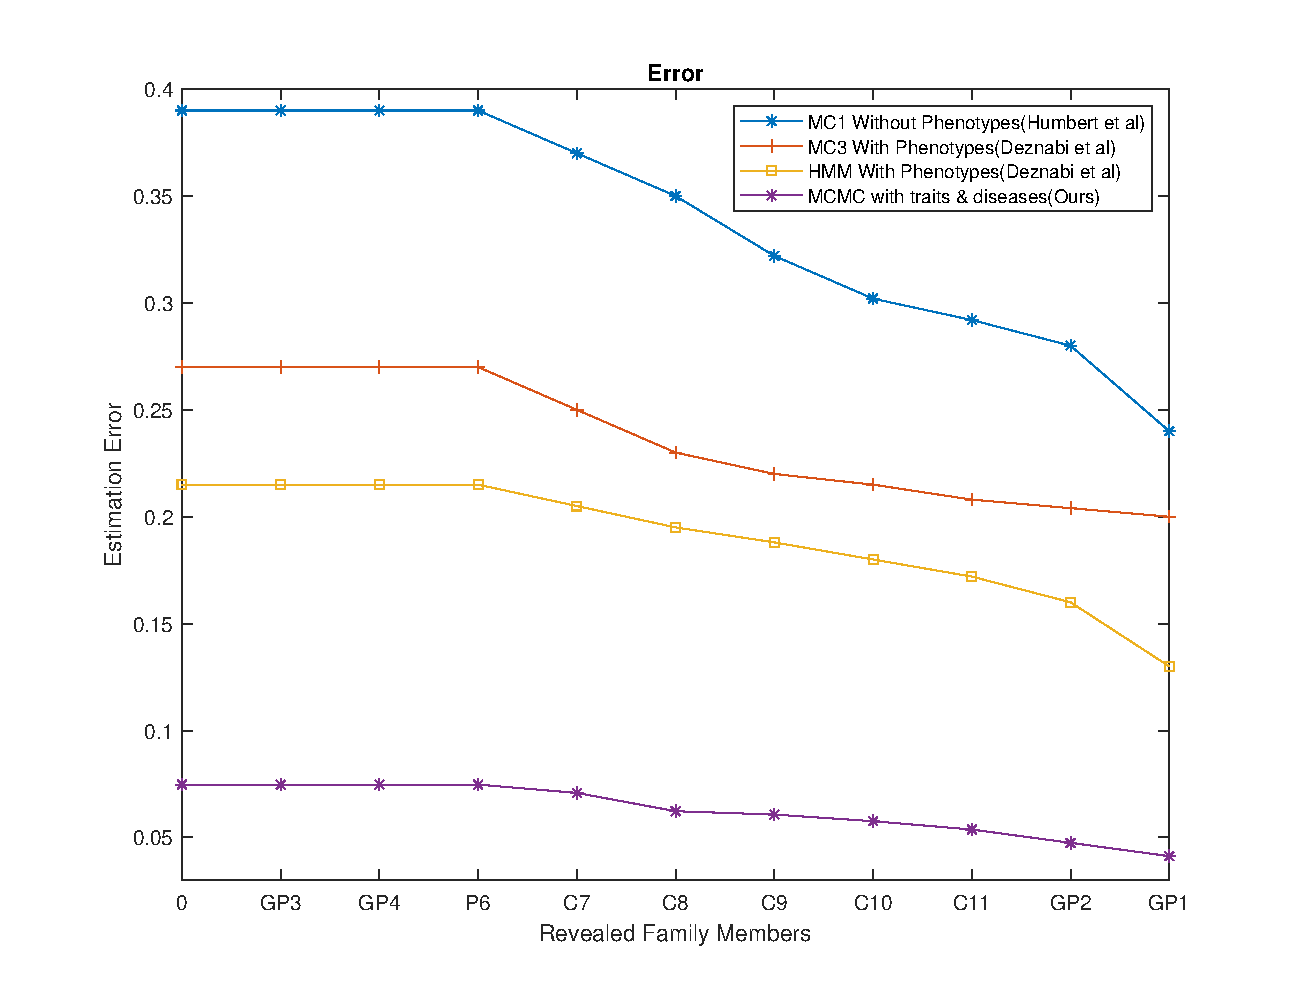
\includegraphics[width=0.8\linewidth]{./figures/P5error1.eps}
	\centering
	\caption{攻击者对P5的SNP序列值属性隐私推断错误率下降情况对比}\label{fig:P5error1}
\end{figure}


我们开始披露观测到的家庭成员中50\%的SNP序列数据,并考察所提出的基因序列属性隐私分析推断攻击的强度。在文献~\cite{humbert2013addressing,humbert2017quantifying}和~\cite{deznabi2018inference}中观测到的家庭成员的SNP序列数据披露顺序是相同的,即从P5的亲属关系最远的一个成员到最亲近的一个成员。 我们分别在图~\ref{fig:P5error1}和图~\ref{fig:P5entropy1}中显示了当50\%SNP序列值被随机隐藏时,先后披露不同家族成员SNP序列数据,攻击者对被攻击者的SNP序列取值的错误率和不确定性递减的结果。 图中,MC1(一阶Markov链或成对连锁不平衡) 代表了Humbert等为考虑基因表型信息情况下的先前工作;MC4(4阶Markov链)代表了Deznabi等的工作,其考虑了基因表型信息,应用了简单隐Markov模型。MCMC(用Markov链Monte Carlo改进隐Markov链)代表了本章的工作,应用了特征和疾病信息。本章工作在攻击者的不正确性和不确定性方面都大大提升了基因属性隐私分析推断攻击的强度。当50\%SNP序列值被随机隐藏时,先后披露不同家族成员SNP序列数据,攻击者获得的基因组隐私递增情况 如图~\ref{fig:P5privacyloss1}所示,它与图~\ref{fig:P5error1}和图~\ref{fig:P5entropy1}中所示的前两个度量指标一致。随着更多的亲属向敌手披露个人基因序列数据,被攻击者泄露给敌手的个人基因序列隐私也会越多。

\begin{figure}[htbp]
	\centering
	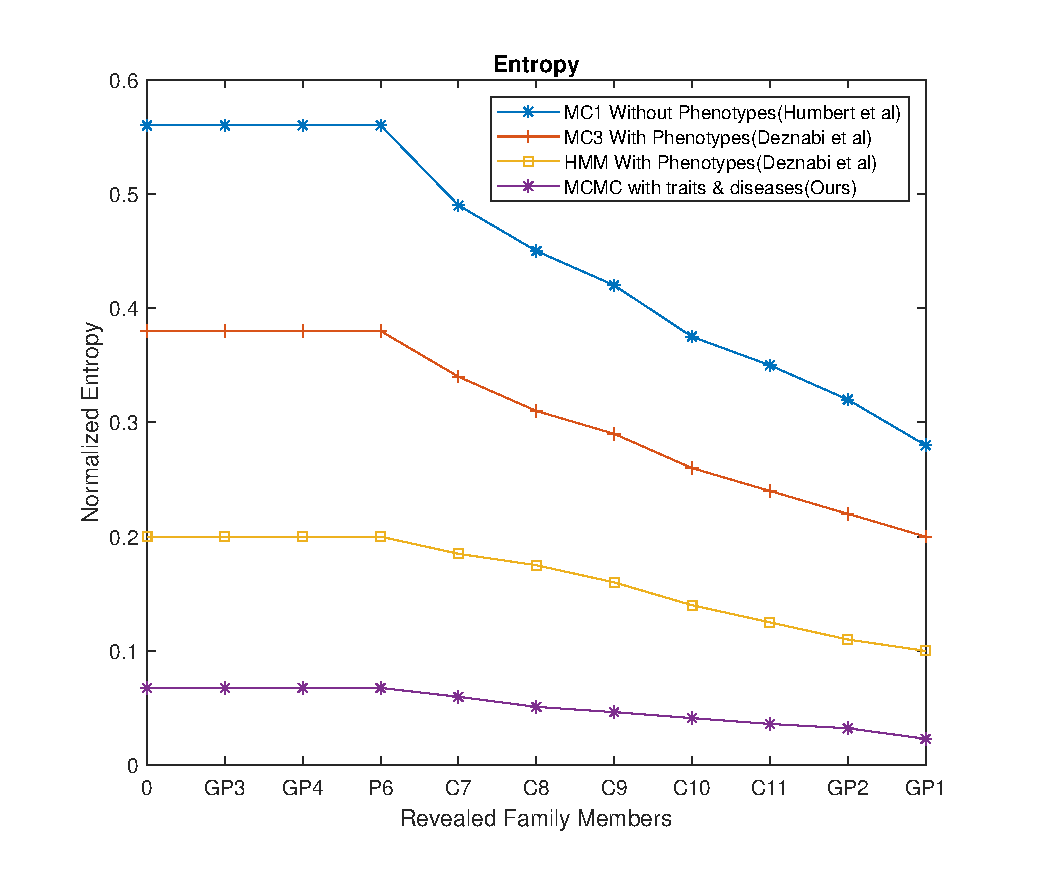
\includegraphics[width=0.8\linewidth]{./figures/P5entropy1.eps}
	\centering
	\caption{攻击者对P5的SNP序列值属性隐私推断不确定性下降情况对比}\label{fig:P5entropy1}
\end{figure}

\begin{figure}[htbp]
	\centering
	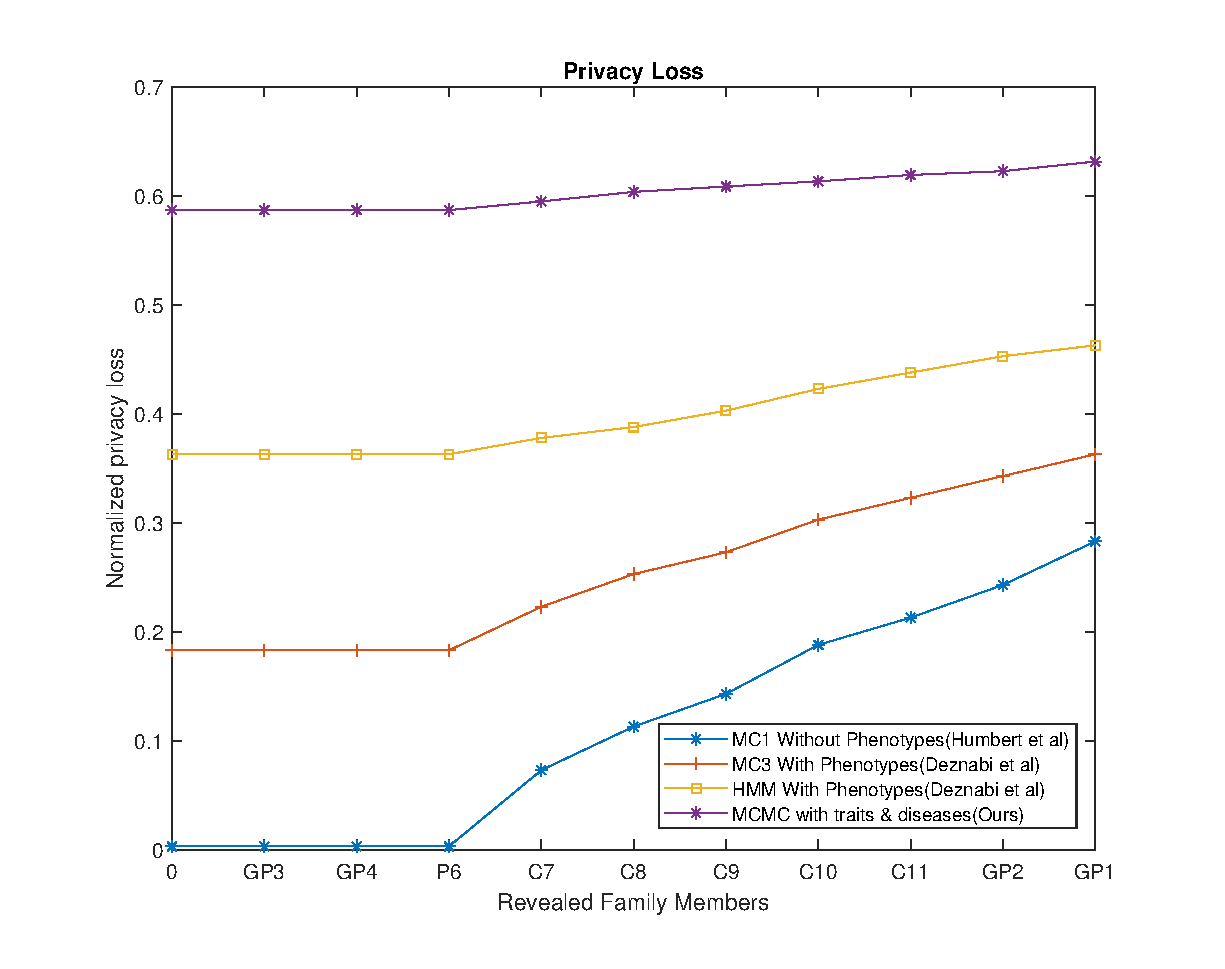
\includegraphics[width=0.8\linewidth]{./figures/P5privacyloss1.eps}
	\centering
	\caption{攻击者对P5的SNP序列值属性隐私推断获取隐私信息量增加情况对比}\label{fig:P5privacyloss1}
\end{figure}


\begin{figure}[htbp]
	\centering
	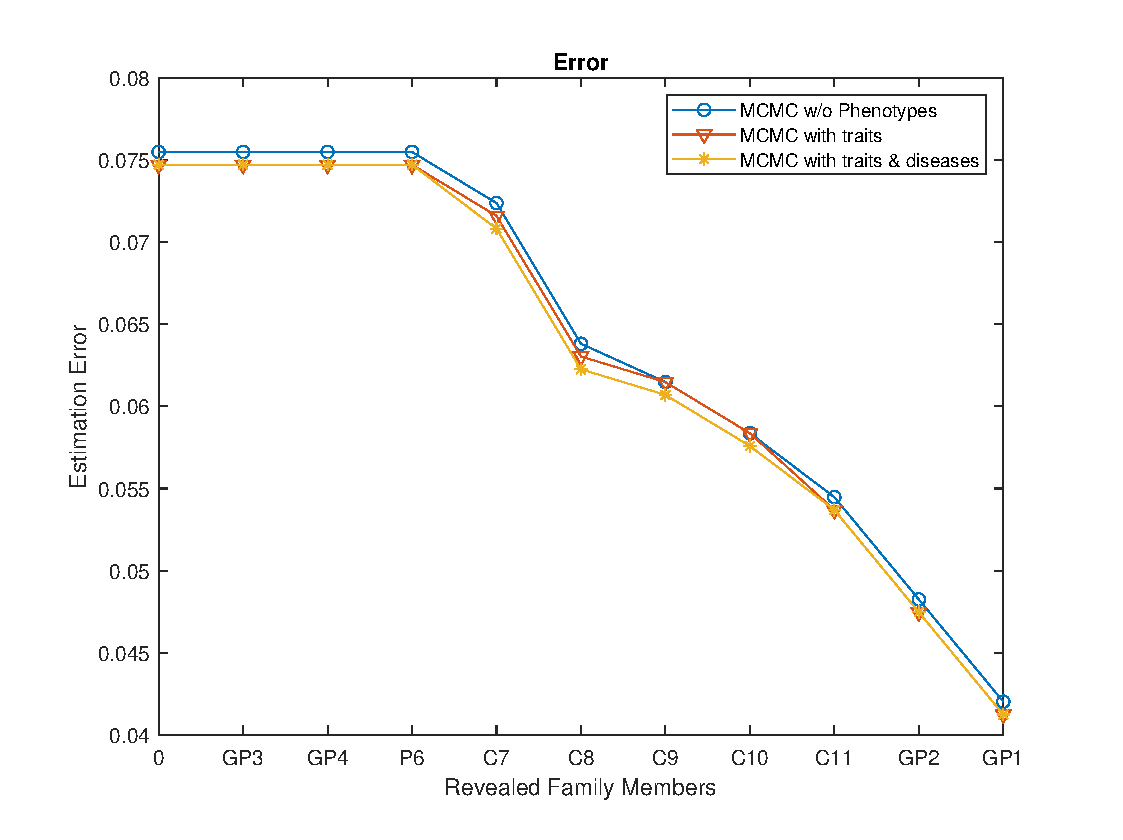
\includegraphics[width=0.8\linewidth]{./figures/P5error2.eps}
	\centering
	\caption{攻击者对P5的SNP序列值属性隐私推断错误率降低情况对比(附加附加特征与疾病信息)}\label{fig:P5error2}
\end{figure}


接下来,为了考察基因表征信息和疾病信息的对被攻击者基因序列属性隐私泄露的影响情况,我们针对提出的推断攻击模型进行了各种附加信息的实验。随机隐藏50\%SNP序列值,先后披露不同家族成员SNP序列数据、相关性状和疾病信息,攻击者对被攻击者的SNP序列取值推断结果的错误率和不确定性递减对比情况如图~\ref{fig:P5error2}和图~\ref{fig:P5entropy2}所示,可以看出攻击者获得的被观测家庭成员的信息越多,被攻击者向攻击者泄露的基因组隐私就越多。

\begin{figure}[htbp]
	\centering
	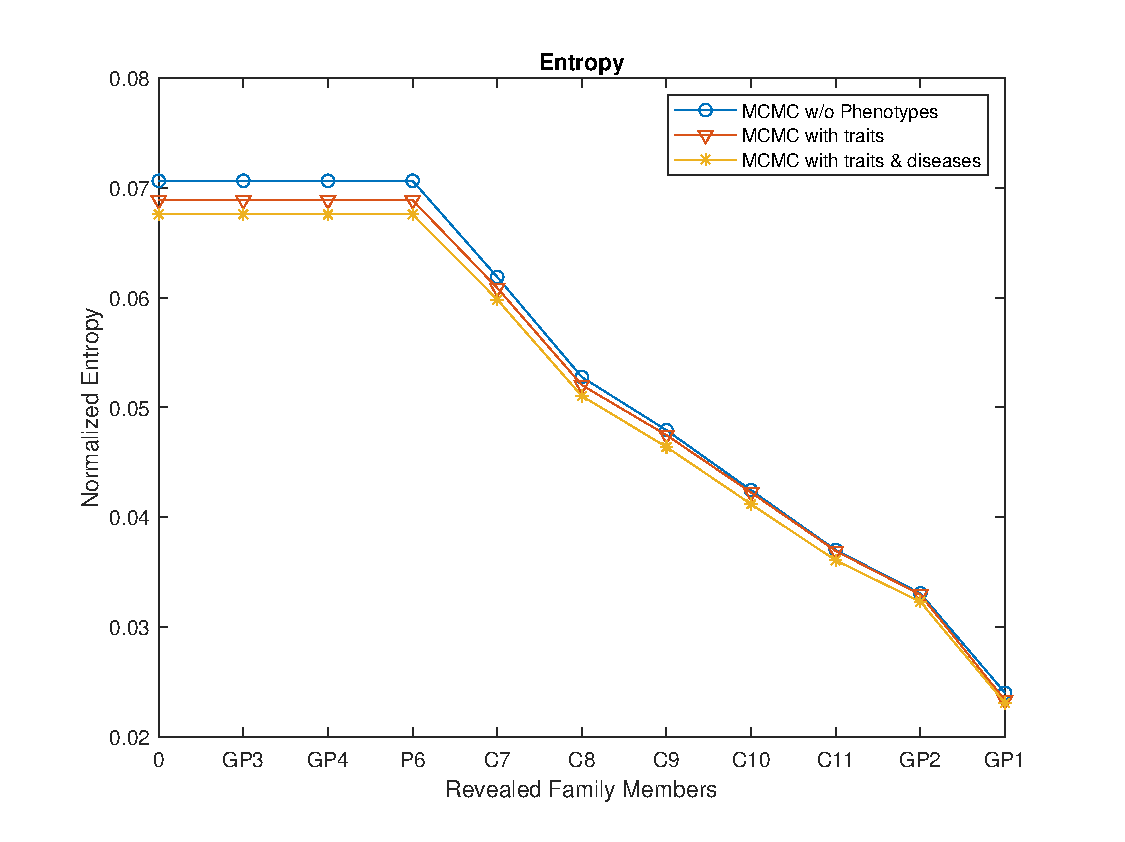
\includegraphics[width=0.8\linewidth]{./figures/P5entropy2.eps}
	\centering
	\caption{攻击者对P5的SNP序列值属性隐私推断不确定性降低情况对比(附加附加特征与疾病信息)}\label{fig:P5entropy2}
\end{figure}


然后,为了考察隐藏的SNP数量对推断攻击模型隐私分析推断能力的影响,我们对家族成员的SNP数据披露顺序与先前试验保持一致,隐藏不同数量的SNP数据以重新进行试验。 该实验中,当10\%的SNP序列值被随机隐藏时,随机披露其他家族成员不同数量的SNP数据,观测攻击者对被攻击者基因序列属性值的推断结果。在图~\ref{fig:P5error3}、图~\ref{fig:P5entropy3}和图~\ref{fig:P5privacyloss3}中,结果表明,随着观测到家族成员的SNP增多,推断攻击的推断能力也随之提高,且这三个指标的结果是一致的。

\begin{figure}[htbp]
	\centering
	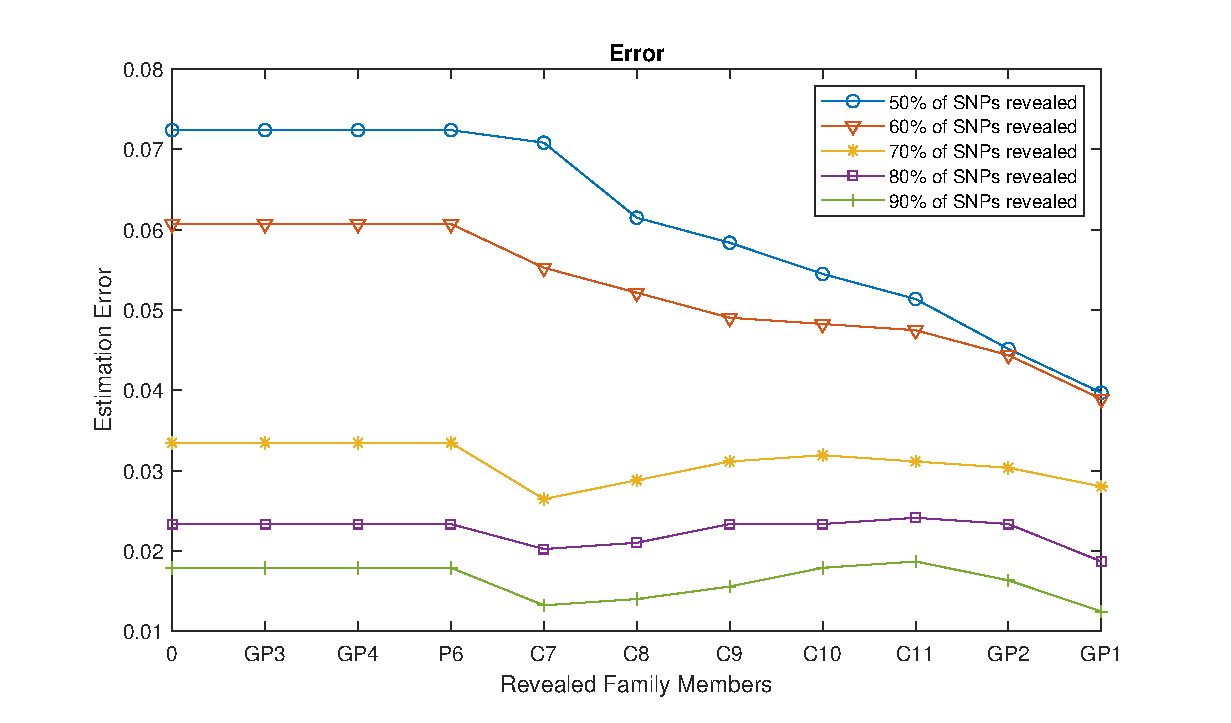
\includegraphics[width=0.8\linewidth]{./figures/P5error3.eps}
	\centering
	\caption{攻击者对P5的SNP序列值属性隐私推断错误率降低情况对比(随机隐藏10\%SNP序列值)}\label{fig:P5error3}
\end{figure}


\begin{figure}[htbp]
	\centering
	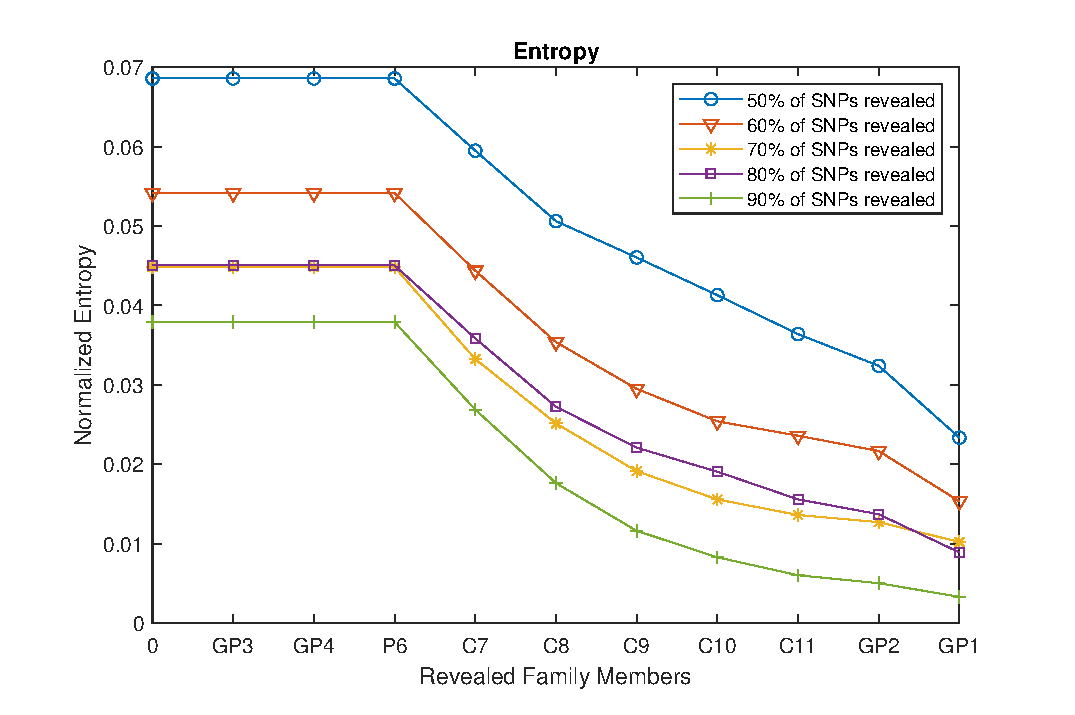
\includegraphics[width=0.8\linewidth]{./figures/P5entropy3.eps}
	\centering
	\caption{攻击者对P5的SNP序列值属性隐私推断不确定性降低情况对比(随机隐藏10\%SNP序列值)}\label{fig:P5entropy3}
\end{figure}

\begin{figure}[htbp]
	\centering
	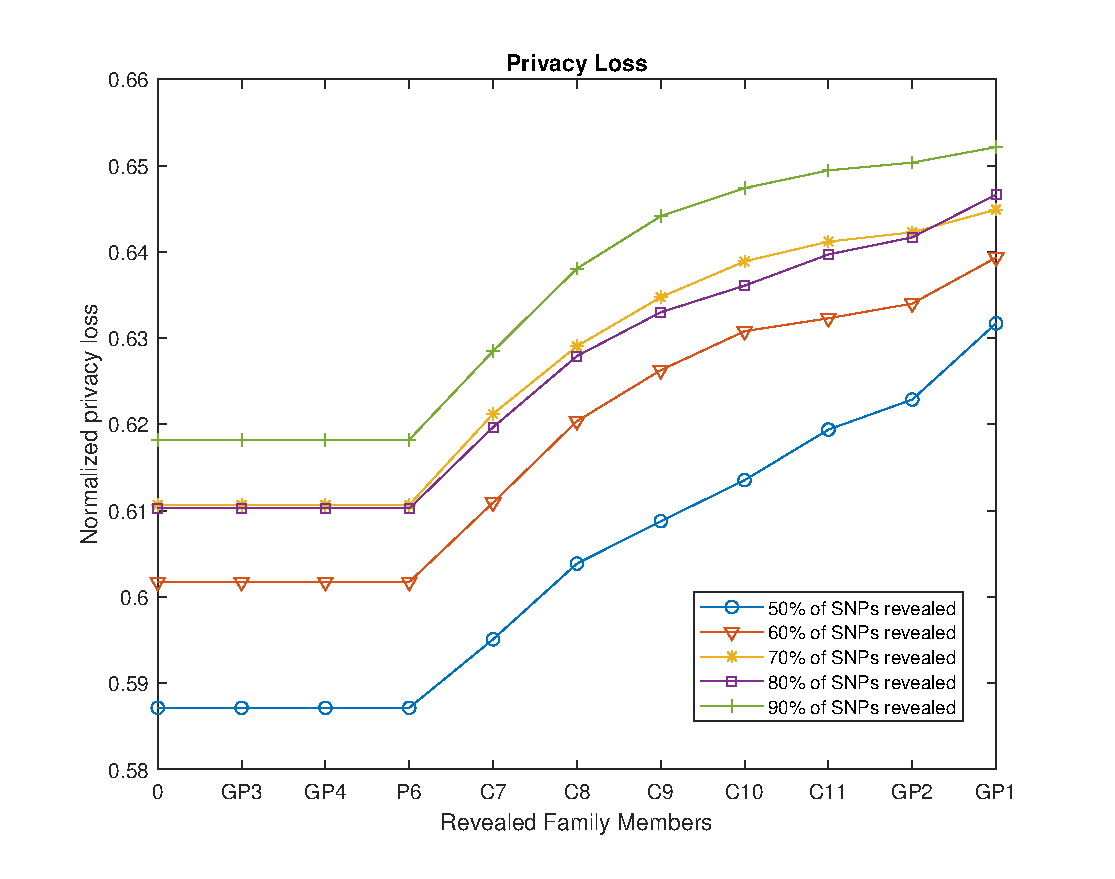
\includegraphics[width=0.8\linewidth]{./figures/P5privacyloss3.eps}
	\centering
	\caption{攻击者对P5的SNP序列值属性隐私推断隐私信息量增加情况对比(随机隐藏10\%SNP序列值)}\label{fig:P5privacyloss3}
\end{figure}


\textbf{(2) Manuel Corpas家族谱系试验结果}

为了与先前的工作保持一致,本章还使用Manuel Corpas家族谱系数据集进行了实验,并将被攻击者设为母亲(图~\ref{fig:Manuel-Corpas-Family-Pedigree}中的M)。 在此实验中,我们开始从M最亲近的家族成员到最远的家族成员进行披露,并分析所提出的基因序列属性隐私分析推断攻击的强度。试验过程中,假设攻击者观测到部分基因组(50\% SNP序列),SNP相关性状(0.3\% SNP序列) 和疾病 (0.4\% SNP序列)信息,攻击者试图推断母亲的基因组序列属性值隐私。

\begin{figure}[htbp]
	\centering
	\includegraphics[width=0.8\linewidth]{./figures/Merror1.eps}
	\centering
	\caption{攻击者对M的SNP序列值属性隐私推断错误率降低情况对比}\label{fig:Merror1}
\end{figure}



\begin{figure}[htbp]
	\centering
	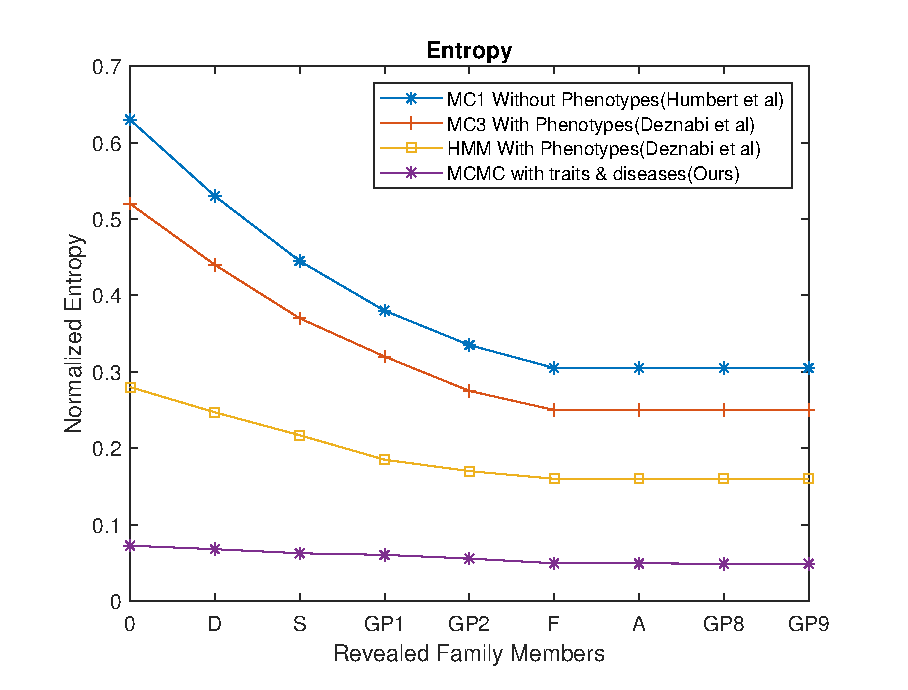
\includegraphics[width=0.8\linewidth]{./figures/Mentropy1.eps}
	\centering
	\caption{攻击者对M的SNP序列值属性隐私推断不确定性降低情况对比}\label{fig:Mentropy}
\end{figure}


随机隐藏50\%SNP序列值,先后披露不同家族成员SNP序列数据、相关性状和疾病信息,攻击者对M的SNP序列值属性隐私推断错误,不确定性和不确定性递减(攻击者获得的基因组隐私量)的结果如图~\ref{fig:Merror1},图~\ref{fig:Mentropy}和图~\ref{fig:Mprivacyloss}所示。结果表明,随着披露SNP序列数据的家族成员数量增加,敌手获取的被攻击者基因序列属性隐私越多,我们所提出的隐私分析推断攻击模型比之前的工作有大幅度提高。此外,试验结果与CEPH/Utah Pedigree 1463数据集的实验结果一致。 敌手对基因序列属性隐私推断攻击的强度取决于披露家庭成员的顺序,这与Deznabi等的工作一致。

\begin{figure}[htbp]
	\centering
	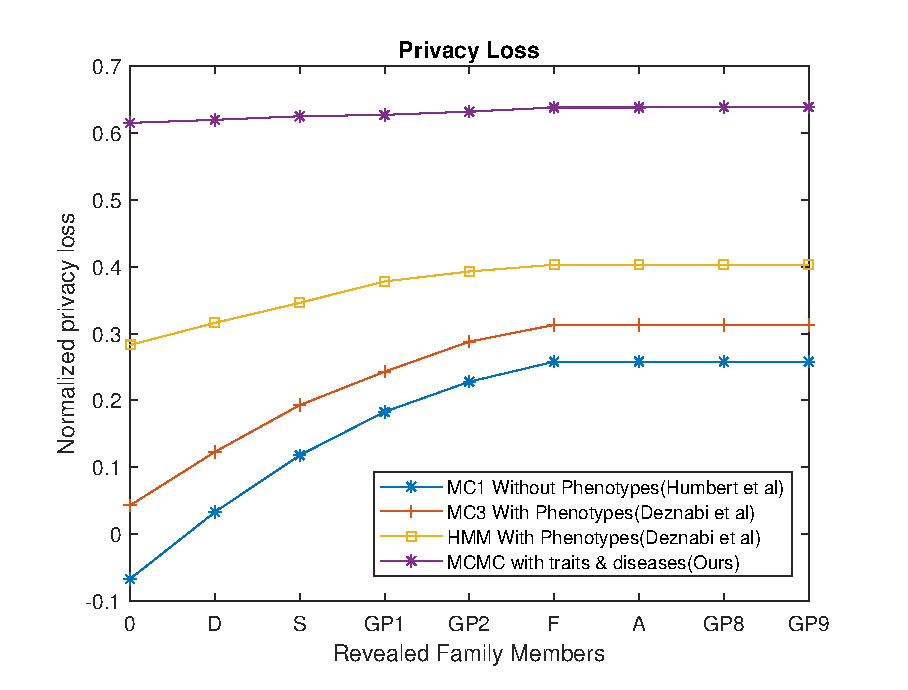
\includegraphics[width=0.8\linewidth]{./figures/Mprivacyloss.eps}
	\centering
	\caption{攻击者对M的SNP序列值属性隐私推断隐私量增加情况对比}\label{fig:Mprivacyloss}
\end{figure}

\section{对比分析}

近年来,有一些针对基因组数据的安全性和隐私问题的工作~\cite{hubaux2017genomic},与本章工作相关的有两类,分别是是基因组补齐和两类基因隐私推断分析。

基因型补齐在基因组关联研究领域被广泛使用~\cite{marchini2007newa},是指通过统计学方法推断未观测到的基因型值。 基因型补齐对在未进行基因型测值的基因标记位评估关联性是非常有用的,且已经有利用不同方法提出的基因型补齐模型相继提出~\cite{howie2009flexible,marchini2007newa,howie2014impute2},但是这些工作旨在提高基因组预测的准确性。 我们的工作集中在基因组数据隐私上,试图推断SNP的敏感值并量化个体的基因组属性隐私。


在文献~\cite{samani2015quantifying} 中,作者提出了对(隐藏)Markov链进行单核苷酸多态性的属性隐私推断攻击模型。 这项工作旨在利用公共信息和观测到的被攻击者的基因组数据推断其自身的基因组隐私。 与文献~\cite{samani2015quantifying}不同,我们试图聚焦在亲属基因组属性隐私问题。 在本章工作中,我们不仅使用了更多的公开基因组信息,例如1000基因组计划数据,孟德尔定律和GWAS目录数据,还使用了被攻击者以外的其他家庭成员的基因组数据。 此外,利用三个度量指标来量化基因组隐私和攻击模型的隐私分析强度。

尽管文献~\cite{humbert2013addressing,humbert2017quantifying}和~\cite{deznabi2018inference}都提出了针对亲属基因组隐私的推断攻击算法,我们与这些工作也存在显着差异,并提高了基因属性隐私推断的准确性。首先,我们针对提出的基因属性隐私推断攻击提出了一个统一的数据和敌手模型,该模型可以刻画不同的基因属性隐私推断攻击算法。其次,在先前的工作中使用错误率和不确定性来量化基因组隐私,我们提出了一种基于互信息的新的基因组隐私量化指标,该指标不仅可以用于量化基因组隐私泄露量,还可以用于评估攻击者的能力;第三,我们采用了基于改进隐Markov链的高阶相关性,而不是朴素的隐Markov链来构建推断攻击模型,且还使用了更多的公共信息来改善推断攻击。第四,我们的工作可以用来攻击高密度SNP序列,而先前的方法仅适用于低密度SNP序列。最后,我们的工作从错误率,不确定性以及隐私损失三方面,提高了相互关联的亲属基因组数据属性隐私推断攻击强度。

\section{小结}

本章中,我们针对相互关联的亲属基因序列数据共享场景,提出了一种基因序列数据属性隐私分析推断模型。该模型利用公开基因组数据,观测到的家庭成员的基因组数据进行基因组属性隐私推断攻击。 本章所提出的关联基因序列属性隐私分析推断模型可以应用于高密度基因数据的隐私分析。基于所提出的隐私分析推断模型和算法,攻击者可以高精度地推断出家族成员中未进行基因数据共享者的SNP序列数据属性值。




	


	

